\documentclass[10pt,a4paper]{article}
\usepackage[utf8]{inputenc}
\usepackage[italian]{babel}
\usepackage{amsmath}
\usepackage{amsfonts}
\usepackage{amssymb}
\usepackage{graphicx}
\usepackage[left=2cm,right=2cm,top=2cm,bottom=2cm]{geometry}
\newcommand{\rem}[1]{[\emph{#1}]}

\author{Gruppo BN \\ Federico Belliardo, Marco Costa, Lisa Bedini}
\title{Semplici circuiti logici e Multivibratori}
\begin{document}

\maketitle
\section{Scopo dell'esperienza}
Nella prima parte dell'esperienza ci si propone di montare e verificare il funzionamento di semplici circuiti logici (AND, OR, XOR e sommatore a un bit) utilizzando solo porte NAND. Successivamente saranno montati un circuito multivibratore monostabile e astabile per verificare la dipendenza lineare tra tempo di durata dell'impulso in uscita e la resistenza presente. Infine questi ultimi due circuiti verranno posti in serie per formare un generatore di onda quadra, per studiare la dipendenza tra le resistenze usate e il \emph{duty cycle}.\\

\section{Materiale occorrente}
\begin{itemize}
\item 2 circuiti integrati SN7400 Quad-NAND Gate;
\item DIP Switch a 4 interruttori;
\item Diodo 1N4148;
\item 2 diodi LED;
\end{itemize}
Disponiamo inoltre del circuito pulsatore montato nella precedente esperienza, costituito da un Arduino Nano e da un octal buffer/driver SN74LS244.

Tutte le resistenze, i condensatori e la tensione di alimentazione sono stati misurati con il multimetro digitale, quindi l'errore è stato propagato secondo le specifiche nel manuale. I tempi e le restanti tensioni sono state misurate con i cursori dell'oscilloscopio: l'errore sui tempi è dato dalla risoluzione dei cursori stessi mentre quello sulle tensioni è stato propagato considerando sia l'errore sul posizionamento dei cursori sia l'errore sistematico del $3\%$.


\section{Semplici circuiti logici}
\subparagraph{Verifica porta NAND}
Abbiamo montato il circuito in figura \ref{fig:NAND}, con una tensione di alimentazione pari a $V_{CC}= 4.85\pm0.03\,\text{V}$, e ne abbiamo verificato il funzionamento prima tramite il diodo LED poi tramite l'oscilloscopio. Si sono usati due interruttori e una resistenza di limitazione di corrente $R_1=327\pm3\,\Omega$. Per mantenere l'input a livello alto anche nel caso di interruttori aperti si è collegato tramite interruttori al ground l'ingresso, dato che di default l'ingresso flottante è riconosciuto come alto. In tabella \ref{tab:NAND} si possono vedere i valori di output attesi: 1 corrisponde al livello alto mentre lo 0 corrisponde al livello basso. Si nota che il LED è spento nel caso di $I_1=I_2=0$ mentre è acceso in tutti gli altri casi. La verifica con l'oscilloscopio si effettua inserendo come input il circuito pulsatore di Arduino\footnote{Abbiamo usato una frequenza di circa 1kHz.}, in questo modo si possono visualizzare tutti gli stati con l'oscilloscopio collegando ad un canale alternativamente l'ingresso $I_1$ e $I_2$., si veda l'immagine \ref{osc:NAND}. Abbiamo usato la traccia di output per il trigger. Nuovamente troviamo la corretta tabella di verità per il NAND.\\


\begin{figure}[!htb]
  \centering
  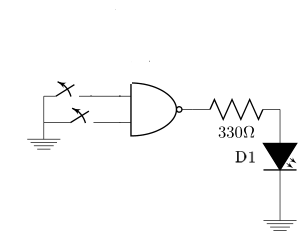
\includegraphics[scale=0.5]{nand.png}
\caption{Schema circuitale della porta NAND.\label{fig:NAND}}
\end{figure}

\begin{table}[!htb]
\centering
\begin{tabular}{|c|c|c|}
\hline 
$I_1$ & $I_2$ & $O$ \\
\hline
 1 &  0 & 1\\ 
 
 1 &  1 & 0\\ 

 0 &  1 & 1\\ 
 
 0 &  0 & 1\\ 
\hline 
\end{tabular} 
\caption{Tabella di verità della porta NAND.\label{tab:NAND}}
\end{table}

\begin{figure}[!htb]
  \centering
  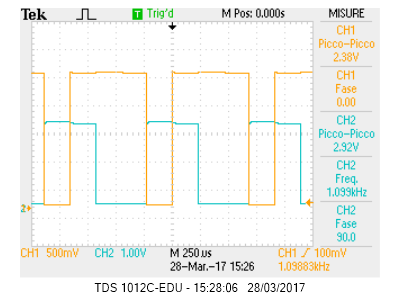
\includegraphics[scale=0.75]{nand1.png}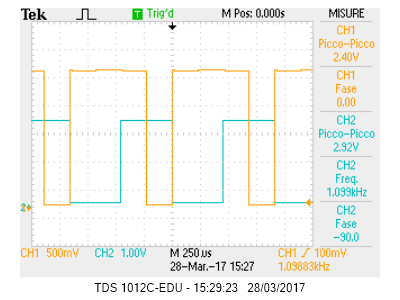
\includegraphics[scale=0.75]{nand2.png}
\caption{Schermate dell'oscilloscopio, in canale 1 c'è l'output e in canale 2 l'input.\label{osc:NAND}}
\end{figure}


\subparagraph{Circuito AND}
E' stato realizzato il circuito in figura \ref{fig:AND}, anche in questo caso si è visualizzato l'output sull'oscilloscopio (figura \ref{osc:AND}), triggerando sul segnale in uscita. Si nota che l'andamento è quello previsto dalla tabella \ref{tab:AND}, infatti nelle immagini fornite dall'oscilloscopio si nota che soltanto quando entrambi gli ingressi sono a livello alto, anche l'uscita è alta.\\

\begin{figure}[!htb]
  \centering
  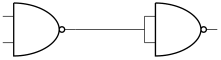
\includegraphics[scale=0.5]{and.png}
\caption{Schema del circuito AND.\label{fig:AND}}
\end{figure}

\begin{table}[!htb]
\centering
\begin{tabular}{|c|c|c|}
\hline 
$I_1$ & $I_2$ & $O$ \\
\hline
 1 &  0 & 0\\ 

 1 &  1 & 1\\ 

 0 &  1 & 0\\ 

 0 &  0 & 0\\ 
\hline 
\end{tabular} 
\caption{Tabella di verità del circuito AND.\label{tab:AND}}
\end{table}

\begin{figure}[!htb]
  \centering
  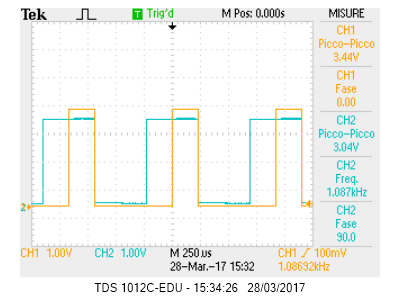
\includegraphics[scale=0.75]{and1.png}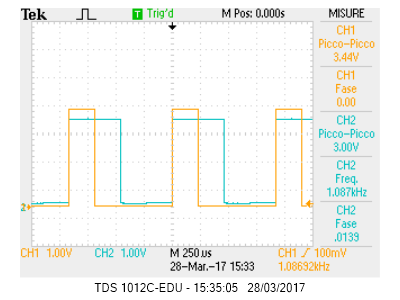
\includegraphics[scale=0.75]{and2.png}
\caption{Schermate dell'oscilloscopio, in canale 1 c'è l'output e in canale 2 l'input.\label{osc:AND}}
\end{figure}

\subparagraph{Circuito OR}

E' stato montato il circuito in figura \ref{fig:OR}. In tabella \ref{tab:OR} è stata rappresentata la tabella di verità e in figura \ref{osc:OR} si può osservare l'andamento dell'output. Si nota che l'uscita è a livello basso quando entrambi gli ingressi sono a 0. Anche in questo caso abbiamo triggerato sull'output e i risultati sono in accordo con la tabella di verità di un OR.

\begin{figure}[!htb]
  \centering
  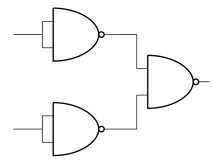
\includegraphics[scale=0.5]{or.png}
\caption{Schema del circuito OR.\label{fig:OR}}
\end{figure}

\begin{table}[!htb]
\begin{tabular}{|c|c|c|}
\hline 
$I_1$ & $I_2$ & $O$ \\
\hline
 1 &  0 & 1\\ 

 1 &  1 & 1\\ 
 
 0 &  1 & 1\\ 
 
 0 &  0 & 0\\ 
\hline 
\end{tabular} 
\caption{Tabella di verità del circuito OR.\label{tab:OR}}
\end{table}

\begin{figure}[!htb]
  \centering
  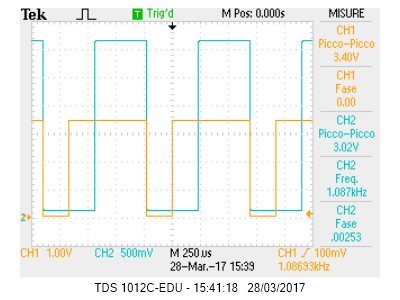
\includegraphics[scale=0.75]{or1.png}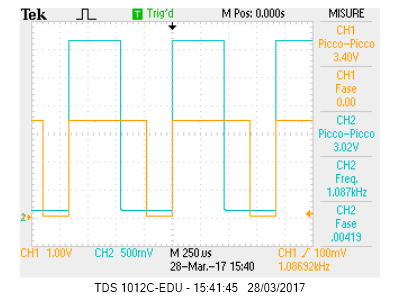
\includegraphics[scale=0.75]{or2.png}
\caption{Schermate dell'oscilloscopio, in canale 1 c'è l'output e in canale 2 l'input.\label{osc:OR}}
\end{figure}

\subparagraph{Circuito XOR}
In questo caso abbiamo dovuto eseguire il trigger su un ingresso perchè la frequenza dell'uscita è doppia rispetto a quella dell'ingresso.


\begin{figure}[!htb]
  \centering
  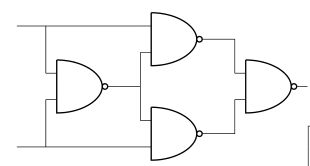
\includegraphics[scale=0.5]{xor.png}
\caption{Schema del circuito XOR.\label{fig:XOR}}
\end{figure}


\begin{table}[!htb]
\centering
\begin{tabular}{|c|c|c|}
\hline 
$I_1$ & $I_2$ & $O$ \\
\hline
 1 &  0 & 1\\ 
 
 1 &  1 & 0\\ 

 0 &  1 & 1\\ 

 0 &  0 & 0\\ 
\hline 
\end{tabular} 
\caption{Tabella di verità del circuito XOR.\label{tab:XOR}}
\end{table}

\begin{figure}[!htb]
  \centering
  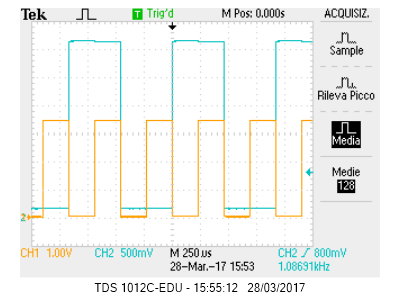
\includegraphics[scale=0.75]{xor1.png}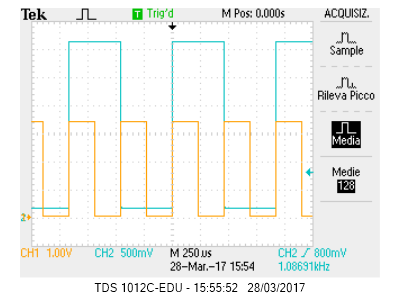
\includegraphics[scale=0.75]{xor2.png}
\caption{Schermate dell'oscilloscopio, in canale 1 c'è l'output e in canale 2 l'input.\label{osc:XOR}}
\end{figure}

\subparagraph{Circuito sommatore a un bit}
Il circuito sommatore a un bit in figura \ref{fig:sommatore} è stato montato aggiungendo al circuito XOR un NOT che preleva il segnale in uscita dal NOT tra i due segnali in ingresso e fornisce l'uscita R. Anche in questo caso abbiamo scritto la tabella di verità (tabella \ref{tab:sommatore}) e visualizzato l'output con l'oscilloscopio (figura \ref{osc:sommatore}). Abbiamo eseguito il trigger sull'uscita R e i risultati sono in accordo con quanto atteso.

%canale 2 R
%canale 1 S e ingressi
%trigger su R


\begin{figure}[!htb]
  \centering
  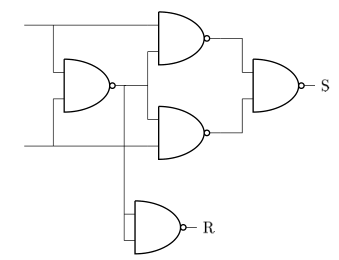
\includegraphics[scale=0.5]{sommatore.png}
\caption{Schema del circuito sommatore a un bit.\label{fig:sommatore}}
\end{figure}

\begin{table}[!htb]
\centering
\begin{tabular}{|c|c|c|c|}
\hline 
$I_1$ & $I_2$ & $S$ & $R$\\
\hline
 1 &  0 & 1 & 0\\ 
 
 1 &  1 & 0 & 1\\ 

 0 &  1 & 1 & 0\\ 
 
 0 &  0 & 0 & 0\\ 
\hline 
\end{tabular} 
\caption{Tabella di verità del circuito sommatore.\label{tab:sommatore}}
\end{table}

\begin{figure}[!htb]
  \centering
  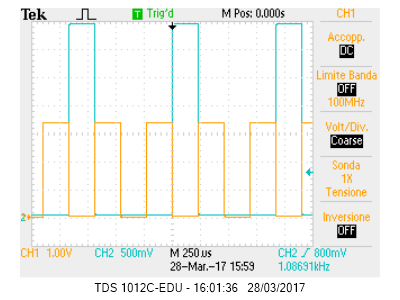
\includegraphics[scale=0.75]{sommatoreRS.png}
\caption{Schermate dell'oscilloscopio, in canale 1 c'è S e in canale 2 R.\label{osc:sommatore}}
\end{figure}

\section{Multivibratore monostabile}
Abbiamo montato il circuito in figura \ref{fig:monostabile}. I componenti sono stati misurati con il multimetro digitale e risultano essere $R_1= 470\pm4\,\Omega$ e $C_1= 110\pm4 \,\text{nF} $. Si è scelta come tensione di alimentazione $V_{CC}= 4.85\pm0.03\,\text{V}$. Si è inviata all'ingresso del circuito tramite generatore di funzioni una onda quadra di frequenza $f = 5.16\pm0.05\,\text{kHz}$. Il periodo risulta quindi pari a $T=194\pm2\,\mu s$ e la durata dell'impulso in uscita%dal generatore di funziomin suppongo
$t=12.8\pm0.2\,\mu s$, ottenendo così un \emph{duty cycle} pari a $6.6\pm0.1\% $. Si è misurata una tensione massima di $4.3\pm0.1\,\text{V}$.
%uppongo questa tensione si il v max del segnale in ingresso 
Abbiamo osservato all'oscilloscopio l'andamento delle tensioni $V_{IN}$, $V_{OUT}$ e $V_{C}$, notando che quando in ingresso si ha l'impulso alto, NAND1 lo interpreta come un 1 quindi all'ingresso di NAND2 si ha uno 0, l'uscita è alta e il condensatore si carica tramite la resistenza $R_1$.\\
Si noti che anche quando il segnale in ingresso è commutatato gli ingressi di NAND2 sono 0 (uscita di NAND3) e 1 (uscita di NAND1) che mantiene a 1 l'uscita. Questo fatto determina l'indipendenza del duty-cyle dal periodo dell'onda in ingresso. A causa della carica di $C_1$, $V_C$ diminuisce esponenzialmente fino a $0$V (la corrente scorre dal condensatore  alla terra dunque non può passare per il diodo ma lo fa sulla resistenza $R1$). $V_C$ diminuisce fino al valore di commutazione $V_C=1.44\pm0.04\,\text{V}$ che corrisponde a $V_{IH}$ per NAND3.\\
 Raggiunto questo valore l'ingresso di NAND3 è interpretato come uno 0 quindi all'ingresso di NAND2 si hanno due 1, pertanto la sua uscita diventa bassa e la tensione $V_C$ diventa negativa poiché  il condensatore ha mantenuto la sua carica (e la differenza di potenziale tra le facce) in questo processo istantaneo, ora per ristabilire l'equilibrio sul condensatore la corrente si scarica attraverso il diodo che entra quindi in interdizione e limita il valore di $V_C$ a $0.80\pm0.02\,\text{V}$.\\
%FIXME (Fede) --> I realtà anche in questa situazine si veede che il valore asintotico d carica e scarica dei condensatori non è 0 ma circa 0.4 (non viene dal diodo) mi chiedo quale sia la ragione.
A questo punto il condensatore si carica finché non arriva un altro impulso. In questo ciclo la carica del condensatore si conserva al variare dei valori logici perché i tempi di commutazione dei NAND sono molto minori dei tempi di carica e scarica di $C_1$. Il tempo atteso caratteristico del circuito RC  infatti è $\tau_{att}=52\pm2\,\mu s$, questo e solo questo valore determina la durata in tempo dell'impulso in uscita.\\
Abbiamo verificato che variando la frequenza in ingresso da circa $33\,kHz$ a circa $10\,kHz$ la durata dell'impulso $t$ in uscita non cambia, mentre si ha una dipendenza di $t$ dalla resistenza. Infatti abbiamo variato il valore della resistenza $R_1$ e misurato la durata dell'impulso, i dati sono presenti in tabella \ref{tab:monostabile}. Per convalidare l'ipotesi di linearità è stato eseguito un \emph{fit} lineare del tipo $t=aR_1+b$ ottenendo i seguenti valori: $a=0.111\pm0.001\,\mu s/\Omega$, $b= -11\pm1\,\mu s$ $\chi^2/ndof=11.57/3$ . Dal grafico in figura \ref{fit:monostabile} è evidente l'andamento lineare eccetto che per gli ultimi punti con un valore della resistenza alto, per cui si ha un aumento del $\chi^2$. Questo è probabilmente dovuto al fatto che l'andamento lineare è apprezzabile se i valori delle resistenze non si discostano troppo da quello di $R_1$, mentre per valori molto maggiori non si può più assumere la linearità a priori.

% periodo T=194\pm2 us
% t up 12.8\pm 0.2 us
%ampiezza in 0.140-4.40 V errore 0.02

%con periodo in 30 ms
%periodo 100 ms

%osservare V_IN, V_C e V_OUT con l'oscilloscopio
% vedere che variando l'impulso input, impulso output non cambia se in è minore di out
%spiegazione teorica e immagini
%cambiare R_1 e fit lineare R_1 vs durata impulso in uscita
%R2 327 ohm
%R3 669 ohm
%R4 824 ohm
%R5 984 ohm
%R6 1.183 kohm
%R7 1.454 kohm

%nand3 commuta quando V_c= 1.44 
%funzione del diodo V_C = 0.8 V
%t_up= 41.60 7pm 0.2 us
%per vedere quando nand3 commuta abbiamo misurato il potenziale vc a cui l'uscita nand 3 cambia di segno

\begin{figure}[!htb]
  \centering
  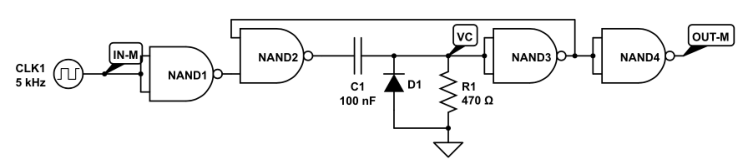
\includegraphics[scale=0.5]{monostabile.png}
\caption{Schema del circuito multivibratore monostabile.\label{fig:monostabile}}
\end{figure}

\begin{table}[!htb]
\centering
\begin{tabular}{|c|c|c|c|}
\hline 
$R_i [\Omega ]$ & $\Delta R_i [\Omega ]$ & $t [\mu s]$ & $\Delta t [\mu s]$\\
\hline
 327 &  3 & 25.8 & 0.2\\ 
\hline 
 470 &  4 & 41.6 & 0.2\\ 
\hline
 669 &  5 & 69.2 & 0.6\\ 
\hline
 824 &  7 & 82 & 1\\ 
\hline 
 984 &  8 & 102 & 1\\ 
\hline
 1183 &  9 & 118 & 1\\ 
\hline
 1454 &  11 & 140 & 1\\ 
\hline
\end{tabular} 
\caption{Presa dati per verificare la linearità fra $R$ e $t$.\label{tab:monostabile}}
\end{table}

\begin{figure}[!htb]
  \centering
  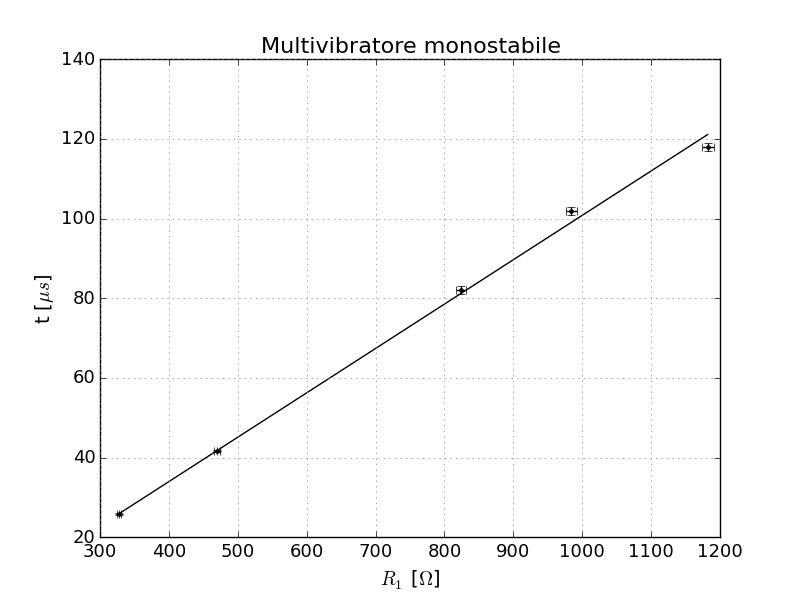
\includegraphics[scale=0.5]{fitmonostabile.png}
\caption{Grafico di t in funzione di $R_1$ e \emph{fit} lineare.\label{fit:monostabile}}
\end{figure}


\section{Multivibratore astabile}
Abbiamo montato il circuito in figura \ref{fig:astabile}, misurando con il multimetro digitale $R_2= 989\pm8\,\Omega$, $C_2= 107\pm4 \,\text{nF} $ e $V_{CC}= 4.85\pm0.03\,\text{V}$. Si sono osservati all'oscilloscopio $V_{C,2}$ e $V_{OUT}$, quindi abbiamo misurato il periodo in uscita $T= 202\pm1\,\mu s $ e $t= 128\pm1,\mu s $, dunque  abbiamo \emph{duty cycle} pari a $63.4\pm0.6\%$. In questo circuito tutte le porte NAND sono usate in configurazione NOT, quindi se l'ingresso di NAND5 è alto, l'uscita di NAND6 è alta e quella di NAND7 è bassa, quindi il condensatore si carica attraverso la resistenza come u un circuito RC in cui il generatore è NAND7 che mantiene una differenza di potenziale tra i suoi estremi. LA situazione asintotica si equlibrio si raggiungerebbe quando la corrente attraverso $R2$ è nulla dunque la tensione $V_{C,2}$ è nulla. Tuttavia la caduta esponenziale della tensione $V_{C,2}$ avviene fino al valore di commutazione $V_{IH}=1.48\pm0.04\,\text{V}$. A questo valore $V_{C,2}$ ha un brusco cambiamento fino a -1.16 V e l'uscita del NAND7 diventa alta, infatti nuovamente la carica sul condensatore si conserva e se l'uscita di NAND6 deve essere bassa allora $V_{C,2}$ deve diventare negativa. Si può immaginare che nel circuto RC equivalente sia istantaneamente invertita l polarità del generatore. Il condensatore si carica e $V_{C,2}$ aumenta fino al valore $1.44\pm0.04\,\text{V}$ quando si ha un altro brusco cambiamento di $V_{C,2}$ e il ciclo si ripete. L'elemento NAND8 serve a rendere il segnale descritto un'onda quadra.

%t=128 \pm1 mus
%T=202\pm1 mus
%vc2 max = 4.08 V
%vc2commutazione out a = 1.48 V
%vC2 min = -1.16 V (simmetrico forse no)
% uscita out positiva quando c si carica fino a 1.44 V perchè è la tensione per cui si passa da livello alto a basso
%ampiezza out 3.52 V

%spiegazione circuito e immagini oscilloscopio
%misurare componenti
Come per il circuito multivibratore monostabile abbiamo variato il valore della resistenza per verificare la dipendenza lineare tra $R_2$ e il periodo in uscita T, quindi abbiamo eseguito un \emph{fit} lineare propagando l'errore sia sulle ascisse che sulle ordinate, figura \ref{fit:astabile} e ottenuto $a=0.195\pm0.003\,\mu s/\Omega$, $b=10\pm3\,\mu s$ e $\chi^2/ndof=5.73/4$.
%tabella e fit

%R 1.788 kohm
%R 2.13 kohm

\begin{table}[!htb]
\centering
\begin{tabular}{|c|c|c|c|}
\hline 
$R_i [\Omega]$ & $\Delta R_i [\Omega]$ & $T [\mu s]$ & $\Delta T [\mu s]$\\
\hline
 669 & 5 & 141  & 1\\ 
\hline
 824 &  7 & 170 & 1\\ 
\hline 
 989 &  8 & 202 & 1\\ 
\hline
 1183 &  9 & 243 & 1\\ 
\hline
 1454 &  11 & 298 & 2\\ 
\hline
 1788 & 14 & 354 & 2 \\
\hline
 2130 & 17 & 446 & 3\\
\end{tabular} 
\caption{Presa dati per verificare la linearità fra $R$ e $T$.\label{tab:astabile}}
\end{table}

\begin{figure}[!htb]
  \centering
  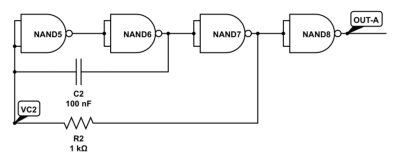
\includegraphics[scale=0.5]{astabile.png}
\caption{Schema del circuito multivibratore astabile.\label{fig:astabile}}
\end{figure}

\begin{figure}[!htb]
  \centering
  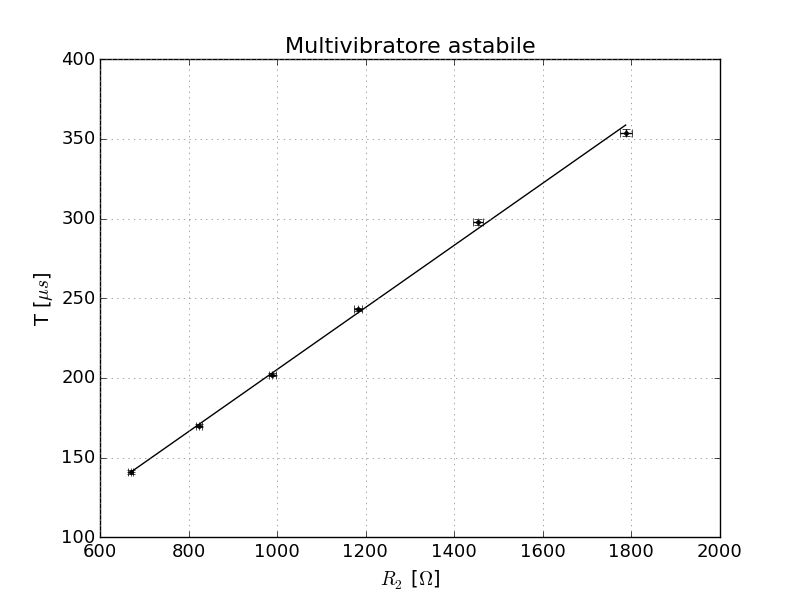
\includegraphics[scale=0.5]{fitastabile.png}
\caption{Grafico di T in funzione di $R_2$ e \emph{fit} lineare.\label{fit:astabile}}
\end{figure}

\section{Generatore di onda quadra}
Il multivibratore astabile è stato collegato al monostabile tramite un derivatore, in modo da ottenere il generatore di onda quadra in figura \ref{fig:generatorequadra}. Si sono usati gli stessi componenti dei circuiti precedenti come $R_1$, $R_2$, $C_1$ e $C_2$ e si sono misurate $R_3=989\pm8\,\Omega$ e $C_3= 10.2\pm0.4 \,\text{nF}$. Da un'analisi qualitativa del circuito si suppone che il periodo dell'onda all'uscita del monostabile dipenda solo dalla costante tempo $\tau_2=C_2R_2$ e che la durata dell'impulso $t$ dipenda solo dalla costante $\tau_1=C_1R_1$. Per verificare questa ipotesi abbiamo cambiato $R_1$ e $R_2$ in modo alternato, i dati sono visibili in tabella \ref{tab:generatore}. Come atteso, cambiando il valore della sola $R_1$ non si hanno variazioni significative del periodo; viceversa, modificando solo il valore di $R_2$ la durata dell'impulso non cambia.
Infine abbiamo stimato i valori delle resistenze per ottenere $T=100\,\mu s$ e \emph{duty cycle} pari al $30\%$, sfruttando le relazioni lineari ottenute dai \emph{fit}: $R_1\simeq $ e $R_2 \simeq $. L'ultima misura presente in tabella \ref{tab:generatore} si riferisce a questa parte e il \emph{duty cycle} relativo risulta pari al TOT

%R2 989
%R3 985 ohm
%C3 10.22 nF

%sensibile al fronte di salita del derivatore, non ai fronti di discesa quindi il monostabile è triggerato dal fronte di salita

outM
%T= 202\pm1 mus
%t= 46\pm1 mus
% V 3.48 V

inM
%offset = 744 \pm 8 mV
%vmax=3.60 V rispetto a 0
%vmin = -1.16 \pm0.05 V
%stima tempo discesa = 7.16 \pm 0.08 mus
%stima 2 tau salita = 5.1\pm0.1

%spiegazione teorica
%immagini




\begin{figure}[!htb]
  \centering
  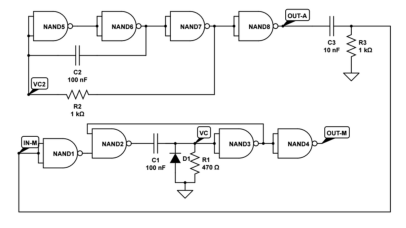
\includegraphics[scale=0.5]{generatorequadra.png}
\caption{Schema del generatore di onda quadra.\label{fig:generatorequadra}}
\end{figure}


%R1 385  328
%R1 = 470; R_2 = 1454; T= 290 \pm 2 mus; t=46.60\pm 0.2 mus
%R_1 = 385; R_2 = 1454; T= 290 \pm 2mus; t=36.0\pm0.2 mus
%R_1= 385; R_2= 1183; T= 238 \pm1 mus; t= 35.8\pm0.2 mus
%R_1=218; R_2=1183; T= 238\pm1 mus;	t= 16.30\pm0.1 mus
%R_1= 218; R_2= 824; T= 171\pm1 mus; t= 16.3\pm0.1
%R_1= 385; R_2= 669; T=	142\pm1 mus;	t=34.6\pm0.2
%R_1=328; R_2= 469; 	T=105\pm 1;	t=	27.6\pm0.2 mus	
%R_1	=385; R_2= 469; T=108\pm1		t=32.8

\begin{table}[!htb]
\centering
\begin{tabular}{|c|c|c|c|c|c|c|c|}
\hline 
$R_{1i} [\Omega]$ & $\Delta R_{1i} [\Omega]$ & $R_{2i} [\Omega]$  & $\Delta R_{2i} [\Omega]$ & $T [\mu s]$ & $\Delta T [\mu s]$&$t [\mu s ]$ & $\Delta t [\mu s]$\\
\hline
 470 & 3 & 1454	& 11 & 290 & 2& 46.6& 0.2\\ 
\hline
385 & 3 & 1454	& 11 & 290 & 2& 36.0& 0.2\\ 
\hline 
 385 & 3 & 1183	& 9 & 238 & 1& 35.8& 0.2\\
\hline
218 & 2 & 1183	& 9 & 238 & 1& 16.3& 0.1\\ 
\hline
218 & 2 & 824	& 7 & 171 & 1& 16.3& 0.1\\ 
\hline
385 & 3 & 669	& 5 & 142 & 1& 34.6& 0.2\\ 
\hline
 385 & 3 & 469	& 3 & 108 & 1& 32.8& 0.2\\ 
 \hline
\end{tabular} 
\caption{Presa dati per verificare la dipendenza della forma d'onda in uscita dalle resistenze.\label{tab:generatore}}
\end{table}

\end{document}